\documentclass[a4paper,10pt]{extarticle}
\usepackage{geometry}
\usepackage[portuguese]{babel}
\usepackage[utf8]{inputenc}
\usepackage[T1]{fontenc}
\usepackage[pdftex]{graphicx}
\newcommand{\NO}{$N^{\underline{o}}\;$}
\newcommand{\ozinho}{$^{\underline{o}}\;$}
\newcommand{\azinho}{$^{\underline{a}}\;$}
%    
\usepackage{xcolor}

\definecolor{orange}{RGB}{255,127,0}
\definecolor{orangered}{RGB}{255,69,0} % Definição
\definecolor{navy}{RGB}{0,0,128}  % cor dos títulos
\definecolor{royalblue}{RGB}{65,105,225} %Exemplo + Obvervação
\definecolor{cyan}{RGB}{0,255,255} %Exemplo + Obvervação
\definecolor{olive}{RGB}{128,128,0} %Exemplo + Obvervação
\definecolor{verde}{RGB}{0,153,0} %Exemplo + Obvervação
\definecolor{amarelo}{RGB}{255,255,0} %Exemplo + Obvervação
\definecolor{laranja}{RGB}{255,128,0} %Exemplo + Obvervação
%
\DeclareSymbolFont{AMSb}{U}{msb}{m}{n}
\DeclareSymbolFontAlphabet{\mathbb}{AMSb}
\def\real {{\mathbb R}}
\def \nat {{\mathbb N}}

\usepackage{times}
\usepackage{enumitem}

\parindent=0pt
\topmargin=-3cm
\oddsidemargin=-2cm
\textwidth=20cm
\textheight=27cm
\renewcommand{\baselinestretch}{1.2}
\pagestyle{empty}
\date{22 de Dezembro de 2020}

\begin{document}
\title{Relatório $-$ \fbox{VERSÃO 55}
}
\author{ André Santos, nº 96152 \and Gustavo Girbal, nº 96226 \and Rogério Henriques, nº 96314 \and Tomás Fonseca, nº 66325}
\maketitle

\paragraph{Percentagem da contribuição para a realização do trabalho de cada elemento do grupo:}
\begin{itemize}
\item André Santos: Grupos: I (33\%), II (10\%), III (40\%)
\item Gustavo Girbal: Grupos: I (33\%), II (10\%), III (40\%)
\item Rogério Henriques: Grupos: I (0\%), II (0\%), III (0\%)
\item Tomás Fonseca: Grupos: I (33\%), II (80\%), III (20\%)
\end{itemize}

\section*{Grupo I}

\begin{enumerate}
\item 
\begin{itemize} 
\item Código da função {\bf newtonquasi}:
{\small
\begin{verbatim}
newtonquasi.m:

function [z, fz, iter] = newtonquasi(f, x0, TolX, MaxIter)
   if nargin < 4 MaxIter = 1e3; end
   if nargin < 3 TolX = 1e-6; end
   iter(1) = x0;
   delta = 1e-5;
   for i = 1:MaxIter
      fz = feval(f, iter(i));
      fd = feval(f, iter(i) + delta);
      fdel = (fd - fz);
      d = (delta*fz) / fdel;
      iter(i+1) = iter(i) - d;
      dif(i) = abs(iter(i+1)-iter(i))/abs(iter(i+1));
      if dif(i) < TolX
	     z = iter(length(iter));
         return
      end
   end   
   fprintf('Maximum number of iterations %d is exceeded\n ', MaxIter); 
   z = iter(length(iter));

\end{verbatim}
}
Código para obter os valores da tabela e o número de iteradas:
{\small
\begin{verbatim}

[z, fz, iter]=newtonquasi(@(x) x^3-x^2-x+1, -0.2, 1e-2, 100)
[z, fz, iter]=newtonquasi(@(x) x^3-x^2-x+1, -0.3, 1e-2, 100)

\end{verbatim}
}
\begin{center}
{\small \begin{tabular}{|c|c|}
\hline
$x_n$&$x_n$\\
\hline
$-0.2000000000000000$&$-0.3000000000000000$\\
\hline
$2.19992000325704$&$8.79867020136542$\\
\hline
$1.69469030681962$&$6.00934048520428$\\
\hline
$1.38700862921966$&$4.16405612789983$\\
\hline 
$1.20801740967179$&$2.95303363047977$\\
\hline
$1.10869034553682$&$2.16996261858035$\\
\hline
$1.05571318850542$&$1.67611842546265$\\
\hline
$1.02823159238950$&$1.37597767220609$\\
\hline
$1.01421589204955$&$1.20177491668567$\\
\hline
$1.00713545758490$&$1.10531038510600$\\
\hline
$$&$1.05394261697684$\\
\hline
$$&$1.02732345448843$\\
\hline
$$&$1.01375570731658$\\
\hline
$$&$1.00690378058862$\\
\hline
\end{tabular}}
\hspace*{10mm}
{\small 
\begin{tabular}{|c|c|c|}
\hline
$x_0$&$-0.2$&$-0.3$\\
\hline
Número de iteradas&$9$&$13$\\
\hline
\end{tabular}}
\end{center}
\end{itemize}
\item 
\begin{enumerate}
\item Código para obter os extremos dos intervalos:
{\small
\begin{verbatim}

[root,fc,k,c,e]=bissecao(@(x) exp(-2*x)*(2*sin(4*x)+cos(4*x))-0.1,0.5,1,1e-15,1e-15,100)

\end{verbatim}

\begin{tabular}{|c|}
\hline
Intervalo\\
\hline
$[0,\; 0.629912674395937]$\\
\hline
\end{tabular}
}
\item 

\begin{itemize}
\item Código para obter os vectores $\bf x$ e $\bf y$, ajuste dos pontos e gráfico da Figura \ref{fig:figura-pergunta1}:
{\small
\begin{verbatim}
grupo1_2b.m:

[root,fc,k,c,e]=bissecao(@(x) exp(-2*x)*(2*sin(4*x)+cos(4*x))-0.001,0.5,1,1e-15,1e-15,100);

[z,fz,iter]=newtonquasi(@(x) exp(-2*x)*(2*sin(4*x)+cos(4*x))-0.001,0.5,1e-12,100);
% com delta = 1e-4

niter=numel(iter);

  for i=1:niter-1
    x(i)=iter(i);
    x(i)=abs(root-x(i));
    x(i)=log(x(i));
  end

  for i=1:niter-1
    y(i)=iter(i+1);
    y(i)=abs(root-y(i));
    y(i)=log(y(i));
  end
  
p=polyfit(x,y,1);
draw=min(x)-20:.1:max(x)+20;
w=polyval(p,draw);
plot(draw,w,x,y,'o','LineWidth',1.2)
xlim([min(x)-10 max(x)+10])
ylim([min(y)-10 max(y)+10])

estimaK=abs((iter(end)-iter(end-1))/(iter(end-1)-iter(end-2)));




\end{verbatim}
}
A recta obtida é $y=A x+B$ com $A=1.15480129631398$ e $B=-3.73811723528024$
\begin{figure}[htb]
\centerline{\scalebox{0.25}{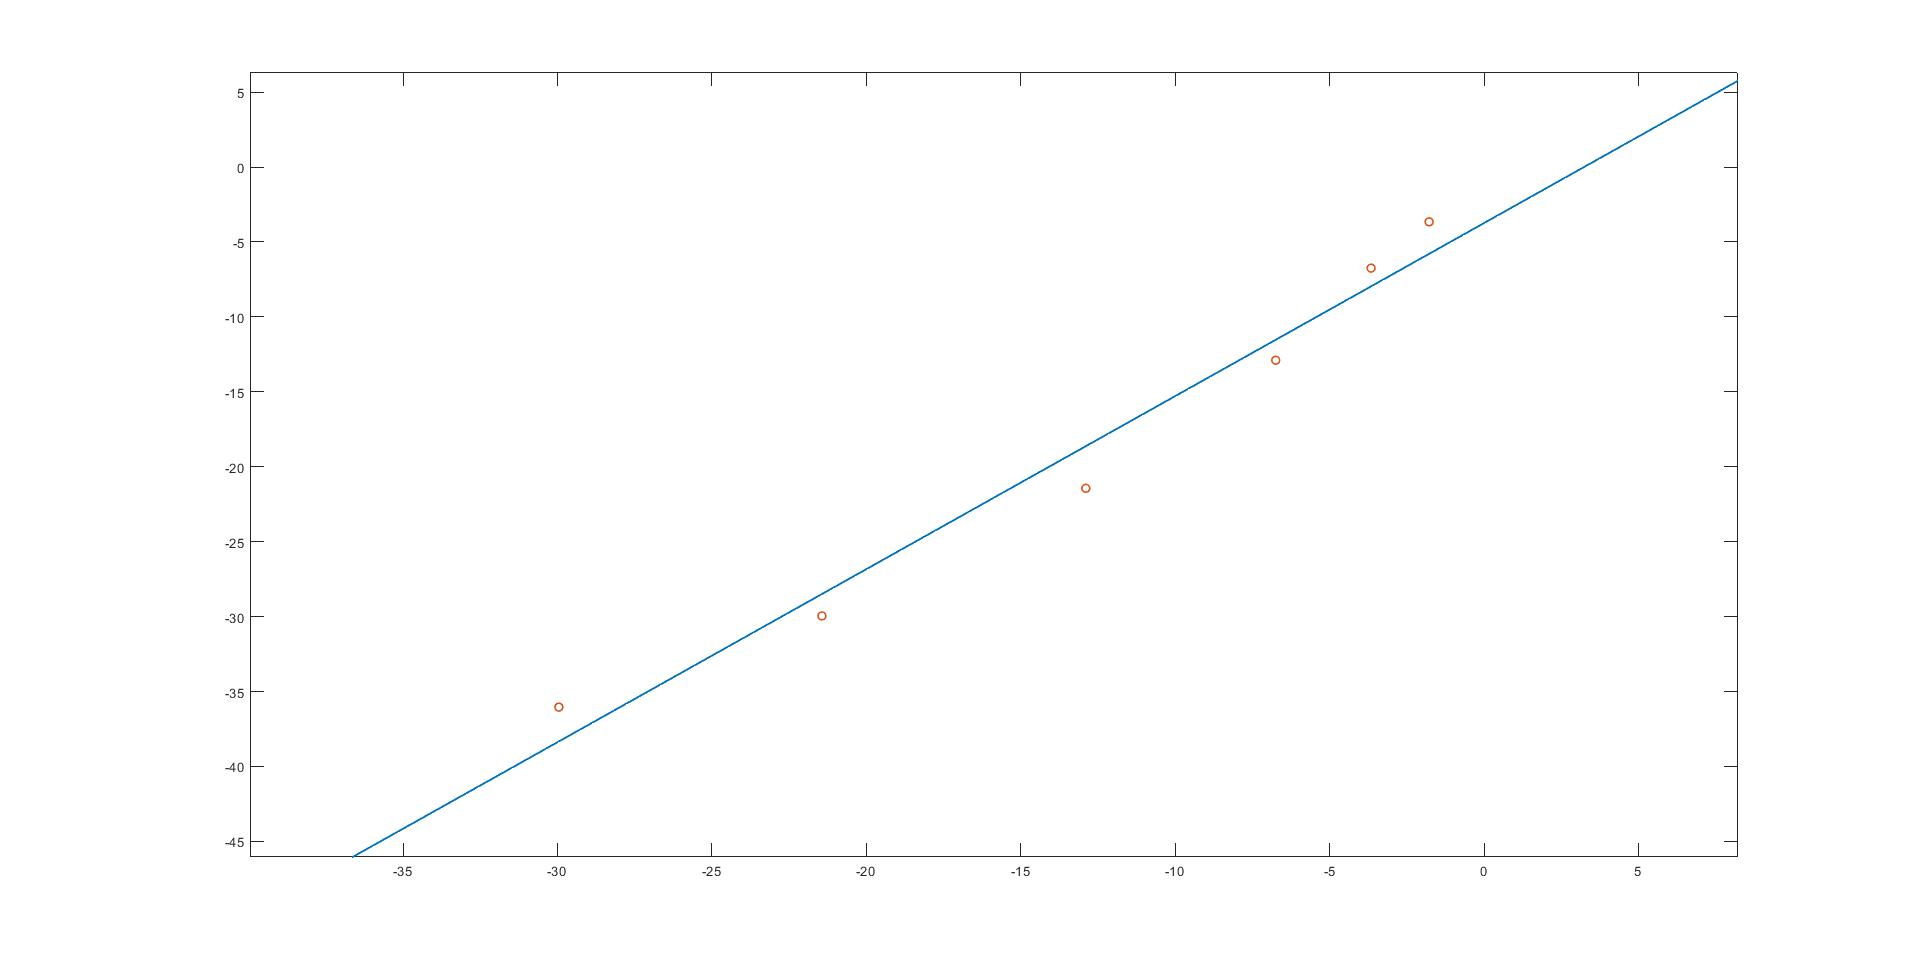
\includegraphics{grafico.jpg}} }
\caption{Gráfico da ordem de convergência.}
\label{fig:figura-pergunta1}
\end{figure}
\item A função iteradora é neste caso
\[x_{n+1}=g(x_n)= x_n-\frac{\delta}{f(\delta+x_n)-f(x_n)}f(x_n)
\]
donde 

\[g'(x)=1-\frac{\delta}{f(\delta+x)-f(x)}f'(x)+\frac{\delta(f'(\delta+x)-f'(x))}{(f(\delta+x)-f(x))^2}f(x)
\]
\[f(x)=e^{-2x}(2sin(4x)+cos(4x))-0.001
\]
\[f'(x)=e^{-2x}(6cos(4x)-8sin(4x))
\]
\[z\approx0.66906
\]
\[f(\delta+z)\approx-2.34606\times 10^{-4}
\]
\[f(z)=0
\]
\[f'(z)\approx-2.34842
\]
logo,
\[g'(z)=1-\frac{\delta}{f(\delta+z)}f'(z)\approx-1.006\times10^{-3}\neq0
\]
pelo teorema da convergência do metodo do ponto fixo, a ordem de convergência é \mbox{1} (linear) e o factor assimptótico de convergência é 
\[K_\infty=1.006\times10^{-3}
\]
A estimativa do coeficiente assimptótico de convergência (utilizando n tanto maior quanto possível) é \mbox{1.995167110566759e-04}
\end{itemize}

\paragraph{Comentário detalhado dos resultados:}

Verificámos que o método de quasi-Newton tem convergência linear, tanto experimentalmente como teoricamente e com o cálculo de uma estimativa. Em todos os estudos de convergência obteve-se um valor do coeficiente assimptótico de convergência próximo de zero, logo é possível prever, que o método tenha uma convergência linear, mas muito próxima de quadrática.
O método de quasi-Newton por nos implementado é, teoricamente, mais lento que o método de Newton, caso este tenha convergência quadrática.

\paragraph{}
\item Código para obter os valores da tabela:
{\small
\begin{verbatim}
grupo1_2c.m:

[root,fc,k,c,e]=bissecao(@(x) exp(-2*x)*(2*sin(4*x)+cos(4*x))-0.001,0.5,1,1e-15,1e-15,100);
[z,fz,iter] = newtonquasi(@(x) exp(-2*x)*(2*sin(4*x)+cos(4*x))-0.001, 0.5, 1e-5, 100);

niter=numel(iter)-1
err=abs(root-z)

\end{verbatim}

}
O $\delta$ mais indicado será o que, simultaneamente terá menor numero de iteradas e erro absoluto. Através da tabela concluimos que $\delta=10^{-6}$.
\begin{center}
{\small \begin{tabular}{|c|c|c|}
\hline
\multicolumn{3}{|c|}{O valor mais apropriado é $\delta=10^{-6}$}\\
\hline
$\delta$&$|e_n|$&Número de iteradas\\
\hline
$10^{-1}$&$7.711622344030999\times 10^{-7}$&$8$\\
\hline
$10^{-2}$&$5.392542412607781\times 10^{-9}$&$5$\\
\hline
$10^{-3}$&$5.901175104128242\times 10^{-10}$&$4$\\
\hline
$10^{-4}$&$4.890274851732102\times 10^{-10}$&$4$\\
\hline
$10^{-5}$&$3.973144035995801\times 10^{-11}$&$4$\\
\hline
$10^{-6}$&$9.754197449751700\times 10^{-12}$&$4$\\
\hline
$10^{-7}$&$1.474709243609595\times 10^{-11}$&$4$\\
\hline
$10^{-8}$&$1.526234694182449\times 10^{-11}$&$4$\\
\hline
$10^{-9}$&$1.520528147835876\times 10^{-11}$&$4$\\
\hline
$10^{-10}$&$1.528022153252095\times 10^{-11}$&$4$\\
\hline
$10^{-11}$&$1.459743437237648\times 10^{-11}$&$4$\\
\hline
$10^{-12}$&$9.844902670863576\times 10^{-12}$&$4$\\
\hline
$10^{-13}$&$1.119228376644799\times 10^{-9}$&$4$\\
\hline
$10^{-14}$&$3.989078511956734\times 10^{-9}$&$4$\\
\hline
\end{tabular}}
\end{center}

\end{enumerate}
\end{enumerate}

\section*{Grupo II}

Código para obter as funções aproximadores, os valores da tabela e o gráfico da 
Figura \ref{fig:figurapergunta2} em formato {\tt .jpg}:
{\small
\begin{verbatim}
grupo2.m:

xdata = 0:.25:3;
ydata = [0.652 0.217 0.264 0.0689 -0.183 0.209 0.529 0.689 1.18 1.48 2.21 3.09 3.64];
draw = xdata(1)-2:.0001:xdata(end)+2;
n = numel(xdata);
tab = zeros(10,4);
mmax = 11;
pval = zeros(mmax,n);
gl = zeros(1,mmax);

for m = 0:mmax
    coef{m+1} = polyfit(xdata,ydata,m);
    pval(m+1,:) = polyval(coef{m+1},xdata);
    w = polyval(coef{m+1},draw);
    tab(m+1,1)=m;
    gl(m+1) = n-(m+1);
    tab(m+1,2) = sum((ydata-pval(m+1,:)).^2);
    tab(m+1,3) = tab(m+1,2)/gl(m+1);
    txt=['Grau ',num2str(m)];
    
    if m <= (mmax/2)
       subplot(1,2,1);
       plot(draw,w,'DisplayName',txt,'LineWidth',1.12);
       hold on
    else
       subplot(1,2,2);
       plot(draw,w,'DisplayName',txt,'LineWidth',1.12);
       hold on
    end
    
    xlim([-.5 3.5])
    ylim([-1 4.5])
    legend show
    legend('Location',"northwest")    
end

for m = 0:(mmax-1)
tab(m+1,4) = tab(m+1,3)/tab(m+2,3);
end

subplot(1,2,1);
plot(xdata,ydata,'o','LineWidth',1.12,'DisplayName','f(x)')
xlabel('x')
ylabel('y')
hold off
subplot(1,2,2);
plot(xdata,ydata,'o','LineWidth',1.12,'DisplayName','f(x)')
xlabel('x')
ylabel('y')
hold off
tab

\end{verbatim}
}
\begin{center}
{\small \begin{tabular}{|c|c|c|c|}
\hline
grau $m$ do polinómio &$\mathrm{SSE}_m$&$\mathrm{MSE}_m$&$\mathrm{MSE}_m/\mathrm{MSE}_{m+1}$\\
\hline
$0$&$17.4670$&$1.4556$&$3.1634$\\
\hline
$1$&$5.0615$&$0.4601$&$26.9990$\\
\hline
$2$&$0.1704$&$0.0170$&$0.9230$\\
\hline
$3$&$0.1662$&$0.0185$&$0.8891$\\
\hline
$4$&$0.1661$&$0.0208$&$0.8858$\\
\hline
$5$&$0.1641$&$0.0234$&$1.0000$\\
\hline
$6$&$0.1407$&$0.0234$&$1.6167$\\
\hline
$7$&$0.0725$&$0.0145$&$1.2410$\\
\hline
$8$&$0.0467$&$0.0117$&$0.8841$\\
\hline
$9$&$0.0397$&$0.0132$&$0.6863$\\
\hline
$10$&$0.0385 $&$0.0193$&$15.3622$\\
\hline
$11$&$0.0013$&$0.0013$&$0$\\
\hline
\end{tabular}
}
\end{center}
\begin{figure}[htb]
\centerline{\scalebox{0.35}{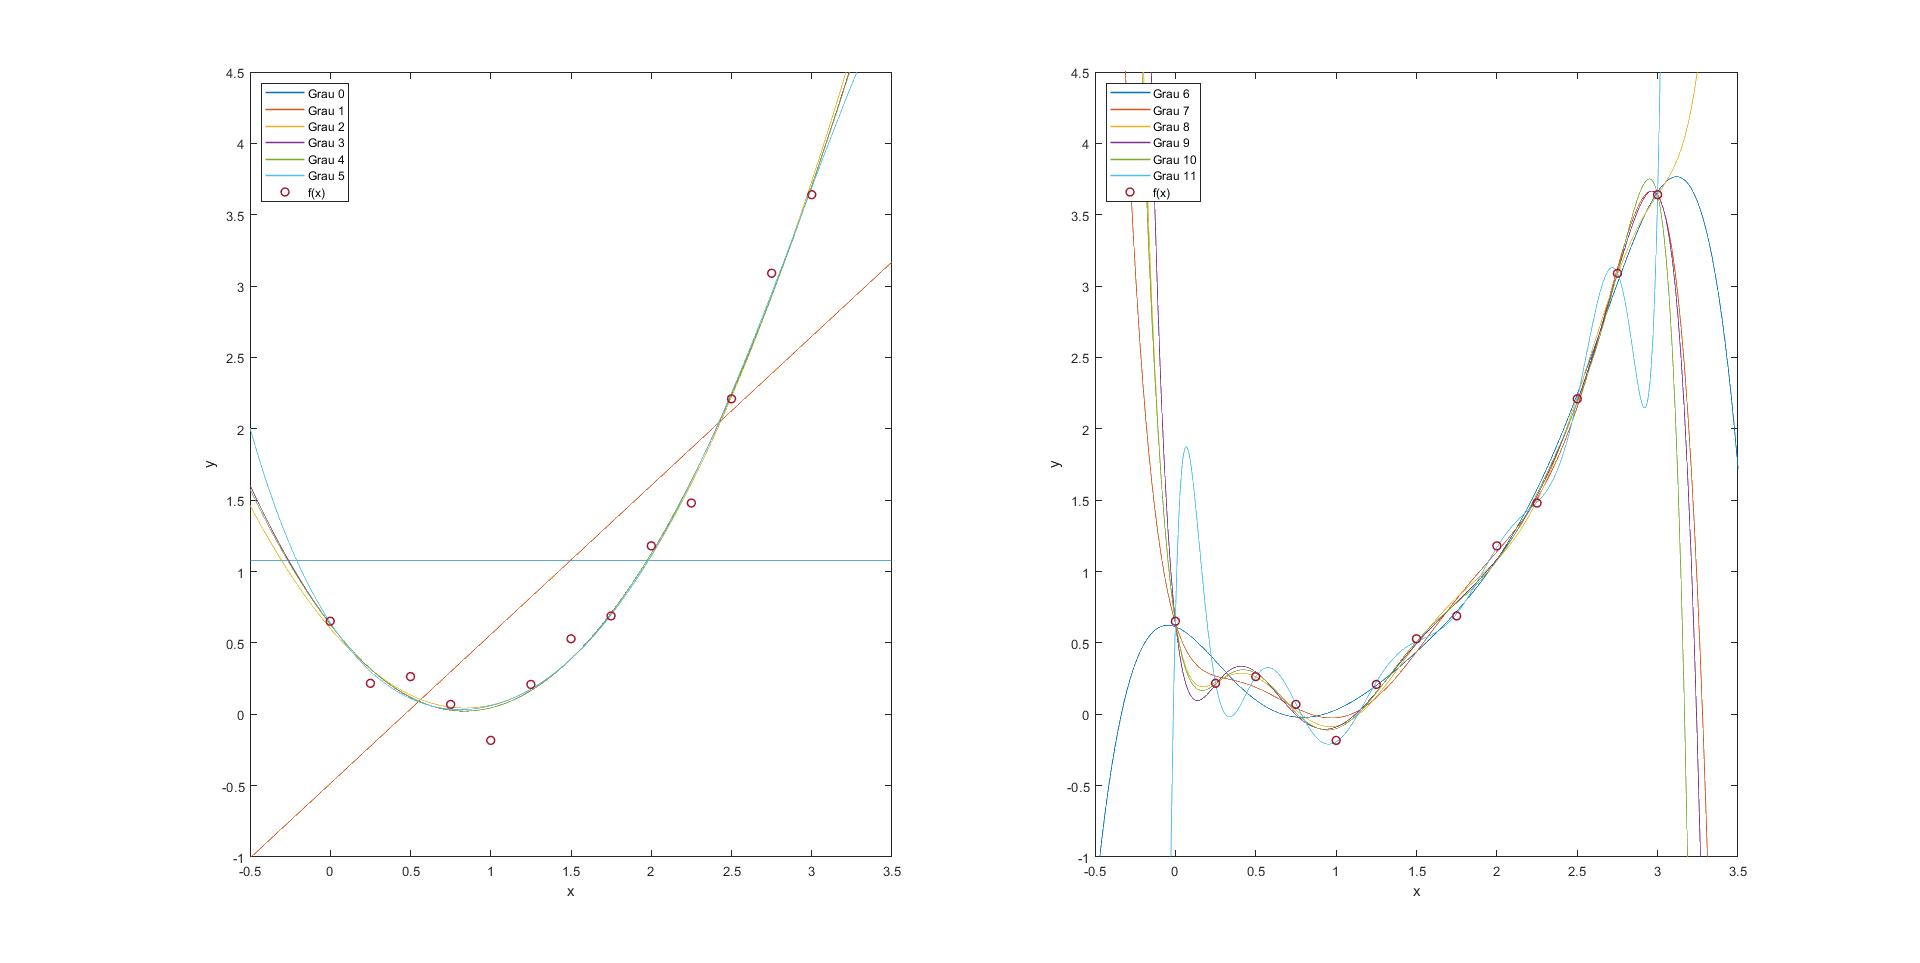
\includegraphics{graficosidebyside.jpg}} }
\caption{Pontos e funções aproximadoras.}
\label{fig:figurapergunta2}
\end{figure}

\paragraph{Justificação da escolha do modelo:}


Após analisar os gráficos da Fig.2, é claro que, qualquer um dos polinómios de grau superior a 5 seria uma má escolha de ajuste apesar do baixo SSE e MSE, isto porque se quisermos prever valores fora da nossa região experimental iremos possivelmente obter estimativas não condizentes com a tendência dos valores observados. Os polinómios de grau muito elevado apresentam um comportamento semelhante ao de um polinómio interpolador para valores fora do intervalo da nossa amostra. Descartamos, também, imediatamente o polinómio de grau 0 e 1, pois possuem SSE bastante elevado.
Resta então analisar os polinómios de grau de 2 a 5. Através da tabela, é possível verificar que todos estes polinómios possuem um SSE semelhante e aceitável e têm um comportamento semelhante na região experimental, contudo se considerarmos os rácios entre os MSE’s, optamos por utilizar o polinómio de grau 2, o mais simples, uma vez que o MSE vai aumentando à medida que se vai aumentando o grau, tornando assim o polinómio de grau dois a escolha mais acertada.
De referir, também, que o modelo escolhido poderia ser ajustado à priori com recurso a um gráfico com os pontos da Tab. 1 representados. Os pontos apresentam um comportamento semelhante a uma parábola, logo o grau do polinómio andaria entre o 2 e 4 para a região amostral.




Modelo escolhido:
\[ P(x)=a_0+a_1x+a_2x^2
\]
Coeficientes que minimizam SSE:
\[a_0=0.6014
\]
\[a_1=-1.3282
\]
\[a_2=0.7908
\]
%\clearpage


\section*{Grupo III}

\begin{enumerate}
\item Código da função {\bf integratrap}:
{\small
\begin{verbatim}
integratrap.m:

function [tab] = integratrap(f,alpha,beta,MaxK)
tab=zeros(MaxK,4);

for k=1:MaxK
n=2^k;  
h=(beta-alpha)/n;
x= alpha:h:beta;
y=feval(f,x);
tab(k,1)=n;
tab(k,2)= trapz(x,y);

   if(k>1)
       tab(k,3)= abs(tab(k,2)-tab(k-1,2));
   end
   
   if(k>2)
       tab(k,4)= abs(tab(k-1,3)/tab(k,3));
   end
   
end

end

\end{verbatim}
}

\item 
\begin{enumerate}
\item Código para obter os gráficos da Figura \ref{fig:figura-perguntaIIIa}
{\small
\begin{verbatim}
grupo3_2a.m:

x1=5:.001:11;
x2=5:.001:(2*pi+5);
x3=5:.001:7;
f1=exp(5-x1).*sin(50.*(x1-5));
f2=1./(2+sin(x2-5));
f3=exp(-x3.^2+10.*x3-25);
subplot(1,3,1);
plot(x1,f1)
xlabel('x')
ylabel('y')
title('exp(5-x)*sin(50*(x-5))')
subplot(1,3,2);
plot(x2,f2)
xlim([5 2*pi+5])
xlabel('x')
ylabel('y')
title('1/(2+sin(x-5))')
subplot(1,3,3);
plot(x3,f3)
xlabel('x')
ylabel('y')
title('exp(-x^2+10*x-25)')

\end{verbatim}
}
\begin{figure}[htb]
\centerline{\scalebox{0.35}{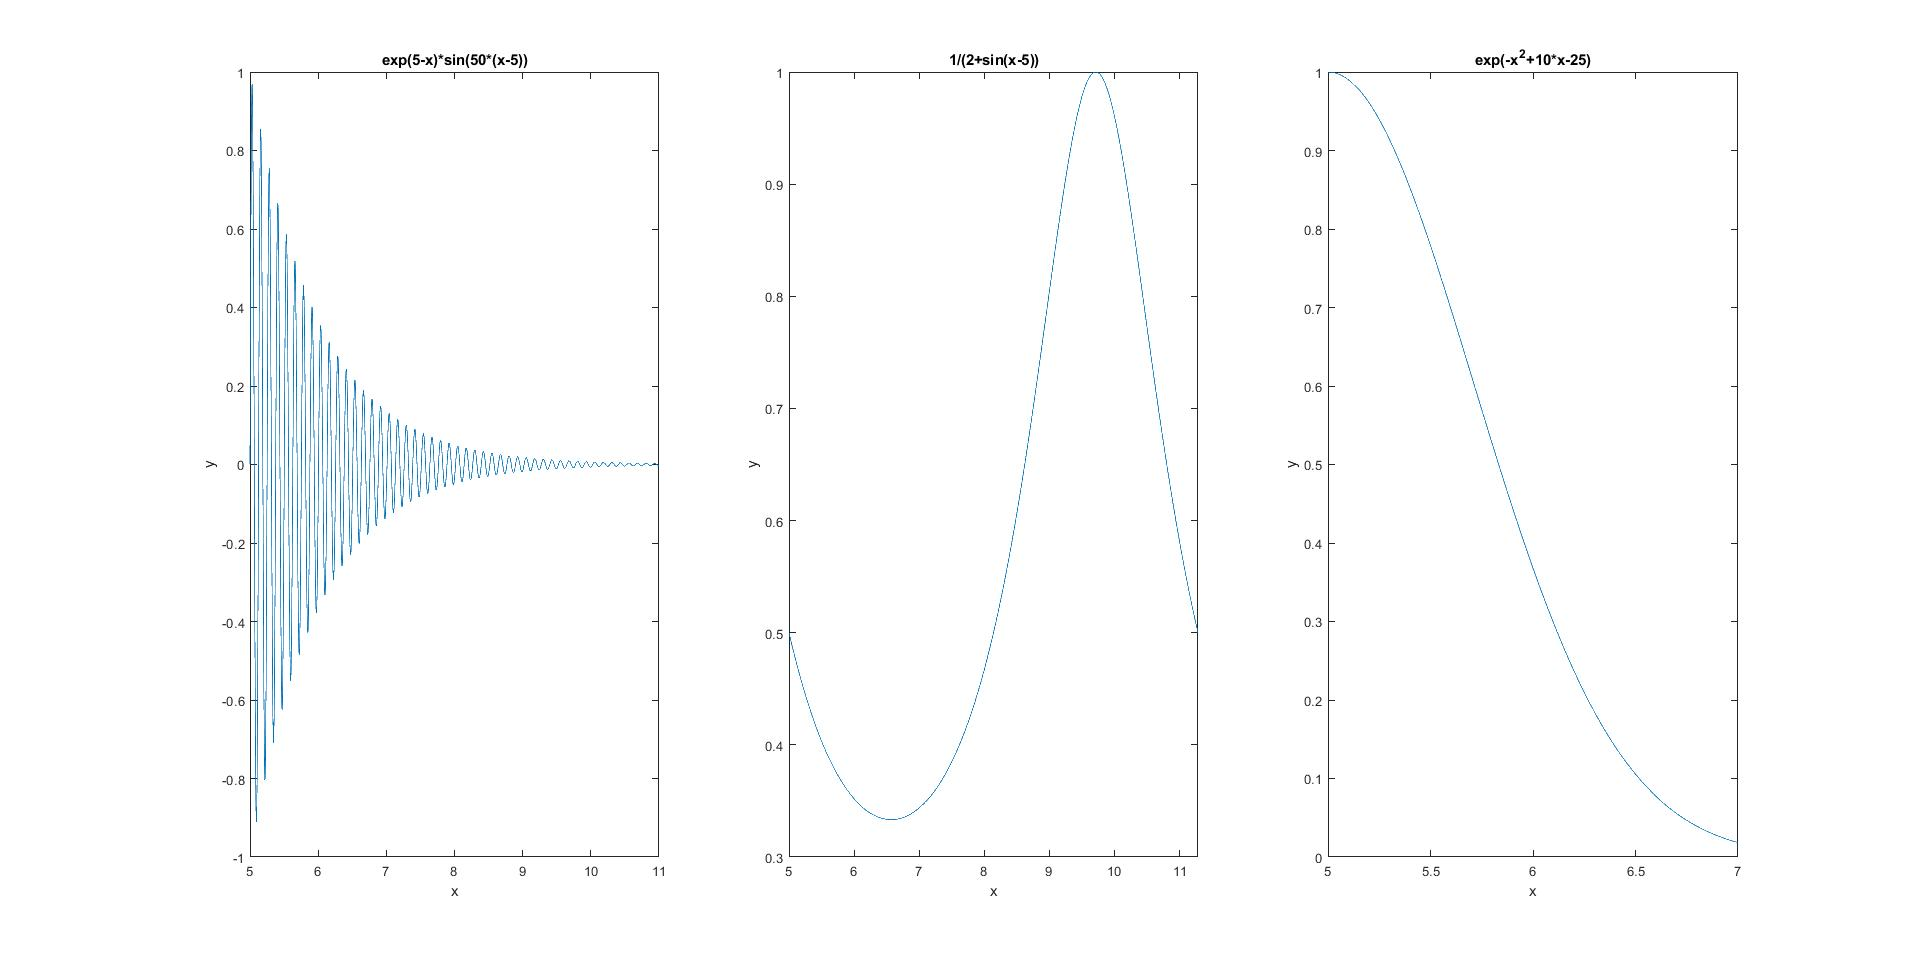
\includegraphics{graficosidebyside3.jpg}} }
\caption{Gráfico das funções integrandas.}
\label{fig:figura-perguntaIIIa}
\end{figure}

\item Código para calcular os valores dos integrais utilizando a função {\bf integratrap}:
{\small
\begin{verbatim}

[tab]=integratrap(@(x)(exp(5-x)).*sin(50.*(x-5)),5,11,19)
[tab]=integratrap(@(x)(2+sin(x-5)).^-1,5,2*pi+5,19)
[tab]=integratrap(@(x)exp((-x.^2)+10*x-25),5,7,19)
















\end{verbatim}
}
Tabela com os valores obtidos:
\begin{center}
{\small\begin{tabular}{|c|c|c|c|}
\hline
\multicolumn{4}{|c|}{Primeiro integral}\\
\hline
 $n$&$T_n$&$|T_{2n}-T_n|$&$|T_{2n}-T_n|/|T_{4n}-T_{2n}|$\\
\hline
 $2$&$-1.104920254759999\times 10^{-1}$&$0$&$0$\\
\hline
 $4$&$-2.005333115252731\times 10^{-1}$&$9.004128604927318\times 10^{-2}$&$0$\\
\hline
 $8$&$-2.334762723742623\times 10^{-1}$&$3.294296084898921\times 10^{-2}$&$2.733248127332062$\\
\hline
$16$&$-2.425825523165001\times 10^{-1}$&$9.106279942237810\times 10^{-3}$&$3.617609062970854 $\\
\hline
$32$&$2.335275830389911\times 10^{-3}$&$2.449178281468900\times 10^{-1}$&$3.718095988004719\times 10^{-2}$\\
\hline
$64$&$-4.551915229915257\times 10^{-2}$&$4.785442812954249\times 10^{-2}$&$5.11797628181648$\\
\hline
$128$&$9.875184325204898\times 10^{-3}$&$5.539433662435747\times 10^{-2}$&$8.638866542270386\times 10^{-1}$\\
\hline
$256$&$1.765117356076460\times 10^{-2}$&$7.775989235559706\times 10^{-3}$&$7.123767143482968$\\
\hline
$512$&$1.941858466744169\times 10^{-2}$&$1.767411106677084\times 10^{-3}$&$4.3996494116071123$\\
\hline
$1024$&$1.985083238254686\times 10^{-2}$&$4.322477151051697\times 10^{-4}$&$4.088884787388770$\\
\hline
$2048$&$1.995831331113539\times 10^{-2}$&$1.074809285885291\times 10^{-4}$&$4.021622447643251$\\
\hline
$4096$&$1.998514752230554\times 10^{-2}$&$2.683421117015417\times 10^{-5}$&$4.005369410973134$\\
\hline
$8192$&$1.999185382830347\times 10^{-2}$&$6.706305997934009\times 10^{-6}$&$4.001340108611343$\\
\hline
$16384$&$1.999353026444872\times 10^{-2}$&$1.676436145243987\times 10^{-6}$&$4.000334887171011$\\
\hline
$32768$&$1.999394936471397\times 10^{-2}$&$4.191002652559339\times 10^{-7}$&$4.000083713190278$\\
\hline
$65536$&$1.999405413923213\times 10^{-2}$&$1.047745181552429\times 10^{-7}$&$4.000020927177725$\\
\hline
$131072$&$1.999408033282739e\times 10^{-2}$&$2.619359526501164\times 10^{-8}$&$4.000005233920541$\\
\hline
$262144$&$1.999408688122409\times 10^{-2}$&$6.548396692951375\times 10^{-9}$&$4.000001296990169$\\
\hline
$524288$&$1.999408851832311\times 10^{-2}$&$1.637099018847454\times 10^{-9}$&$4.000000377229203$\\
\hline
\end{tabular}}
\end{center}
\begin{center}
{\small\begin{tabular}{|c|c|c|c|}
\hline
\multicolumn{4}{|c|}{Segundo integral}\\
\hline
 $n$&$T_n$&$|T_{2n}-T_n|$&$|T_{2n}-T_n|/|T_{4n}-T_{2n}|$\\
\hline
 $2$&$3.141592653589793$&$0$&$0$\\
\hline
 $4$&$3.665191429188092$&$5.235987755982987\times 10^{-1}$&$0$\\
\hline
 $8$&$3.627791516645357$&$3.739991254273489\times 10^{-2}$&$1.400000000000027\times 10^{1}$\\
\hline
$16$&$3.627598733591012$&$1.927830543446696\times 10^{-4}$&$1.939999999993204\times 10^{2}$\\
\hline
$32$&$3.627598728468435$&$5.122577029226250\times 10^{-9}$&$3.763399813116893\times 10^{4}$\\
\hline
$64$&$3.627598728468436$&$4.440892098500626\times 10^{-16}$&$1.153501800000000\times 10^{7}$\\
\hline
$128$&$3.627598728468436$&$0$&$Inf$\\
\hline
$256$&$3.627598728468435$&$4.440892098500626\times 10^{-16}$&$0$\\
\hline
$512$&$3.627598728468436$&$4.440892098500626\times 10^{-16}$&$1$\\
\hline
$1024$&$3.627598728468436$&$0$&$Inf$\\
\hline
$2048$&$3.627598728468436$&$4.440892098500626\times 10^{-16}$&$0$\\
\hline
$4096$&$3.627598728468436$&$4.440892098500626\times 10^{-16}$&$1$\\
\hline
$8192$&$3.627598728468436$&$0$&$Inf$\\
\hline
$16384$&$3.627598728468436$&$0$&$0$\\
\hline
$32768$&$3.627598728468436$&$0$&$1$\\
\hline
$65536$&$3.627598728468436$&$0$&$Inf$\\
\hline
$131072$&$3.627598728468436e$&$0$&$NaN$\\
\hline
$262144$&$3.627598728468436$&$0$&$0$\\
\hline
$524288$&$3.627598728468434$&$1.332267629550188\times 10^{-15}$&$1$\\
\hline
\end{tabular}}
\end{center}
\begin{center}
{\small\begin{tabular}{|c|c|c|c|}
\hline
\multicolumn{4}{|c|}{Terceiro integral}\\
\hline
 $n$&$T_n$&$|T_{2n}-T_n|$&$|T_{2n}-T_n|/|T_{4n}-T_{2n}|$\\
\hline
 $2$&$8.770372606158094\times 10^{-1}$&$0$&$0$\\
\hline
 $4$&$8.806186341245394\times 10^{-1}$&$3.581373508730001\times 10^{-3}$&$0$\\
\hline
 $8$&$8.817037913321336\times 10^{-1}$&$1.085157207594167\times 10^{-3}$&$3.300326886894145$\\
\hline
$16$&$8.819862452657771\times 10^{-1}$&$2.824539336434562\times 10^{-4}$&$3.841890936325107$\\
\hline
$32$&$8.820575578012115\times 10^{-1}$&$7.131253543446459\times 10^{-5}$&$3.960789388887009$\\
\hline
$64$&$8.820754296107940\times 10^{-1}$&$1.787180958245926\times 10^{-5}$&$3.990224666698333$\\
\hline
$128$&$8.820799002925631\times 10^{-1}$&$4.470681769119800\times 10^{-6}$&$3.997557980061264$\\
\hline
$256$&$8.820810181335852\times 10^{-1}$&$1.117841022080235\times 10^{-6}$&$3.999389609803485$\\
\hline
$512$&$8.820812976045018\times 10^{-1}$&$2.794709166309417\times 10^{-7}$&$3.999847410084577$\\
\hline
$1024$&$8.820813674728973\times 10^{-1}$&$6.986839551359481\times 10^{-8}$&$3.999961850799379$\\
\hline
$2048$&$8.820813849400377\times 10^{-1}$&$1.746714040073982\times 10^{-8}$&$3.999990491324815$\\
\hline
$4096$&$8.820813893068254\times 10^{-1}$&$4.366787709209063\times 10^{-9}$&$3.999997610120499$\\
\hline
$8192$&$8.820813903985227\times 10^{-1}$&$1.091697288124749\times 10^{-9}$&$3.999998677939436$\\
\hline
$16384$&$8.820813906714469\times 10^{-1}$&$2.729241277421579\times 10^{-10}$&$4.000002847517087$\\
\hline
$32768$&$8.820813907396781\times 10^{-1}$&$6.823119846899317\times 10^{-11}$&$3.999990237108101$\\
\hline
$65536$&$8.820813907567358\times 10^{-1}$&$1.705768859494583\times 10^{-11}$&$4.000026034547845$\\
\hline
$131072$&$8.820813907610001\times 10^{-1}$&$4.264366637585226\times 10^{-12}$&$4.000052069773496$\\
\hline
$262144$&$8.820813907620664\times 10^{-1}$&$1.066258192850000\times 10^{-12}$&$3.999375260308205$\\
\hline
$524288$&$8.820813907623327\times 10^{-1}$&$2.663425036075751\times 10^{-13}$&$4.003334722801167$\\
\hline
\end{tabular}}
\end{center}

\paragraph{Comentário detalhado:}

Comparativamente a outros métodos de integração, o método dos trapézios não é o mais eficiente. Contudo, chega a valores extramente próximos do real, mostrando a sua precisão. Apesar de não ser o mais eficiente, permite chegar a valores extremamente próximos de integrais que são extremamente difíceis ou até impossíveis de calcular manualmente. Seria de esperar que os valores da quarta linha da segunda tabela tendessem para 4, de modo semelhante ao das tabelas 1 e 3, uma vez que à medida que duplicamos o numero de intervalos, o erro diminui, teoricamente, 4x. O facto de isto não acontecer pode-se dever ao facto de que é encontrado um valor muito próximo do valor real do integral muito rapidamente, resultando em erros absolutos muito próximos de zero e impedindo o quociente de chegar a convergir para o valor teórico.

\item Código para calcular o número mínimo de subintervalos para que o erro seja menor que $10^{-6}$.

{\small
\begin{verbatim}
calculon.m:

function [n] = calculon(tab)
eerr = tab(:,3)./3;
dim = size(eerr);
for i = 2:dim(1)
    if eerr(i) < 1e-6
        n = 2^(i);
        break
    end
end
end

grupo3_2c.m:

[tab]=integratrap(@(x)(exp(5-x)).*sin(50.*(x-5)),5,11,19);
[n1] = calculon(tab)
[tab]=integratrap(@(x)(2+sin(x-5)).^-1,5,2*pi+5,19);
[n2] = calculon(tab)
[tab]=integratrap(@(x)exp((-x.^2)+10*x-25),5,7,19);
[n3] = calculon(tab)

\end{verbatim}
}

{\small 
\begin{center}
\begin{tabular}{|c|c|c|c|}
\hline
& Teórico&Experimental& Teórico $/$ Experimental\\
\hline
1º caso & $208973$&$16384$& $12.755$\\
\hline
2º caso & $4547$&$32$& $142.1$\\
\hline
3º caso & $1155$&$256$& $4.512$\\
\hline
\end{tabular}
\end{center}
}

\paragraph{Comentário detalhado:}

Como era de esperar, o valor do número mínimo de subintervalos experimental é mais pequeno do que o teórico, já que o erro teórico foi calculado através de uma majoração, logo representa o número mínimo de pontos necessários que, teoricamente, garantidamente nos dão uma boa aproximação do valor real do integral. O valor obtido experimentalmente representa um valor calculado e não o extremo, logo é mais baixo.

\end{enumerate}
\end{enumerate}
\section*{Bibliografia}

\begin{description}
\item Isabel Reis dos Santos. 2020. {\it slidesMEEC4to1.pdf}.
\item Isabel Reis dos Santos. 2020. {\it Exercicios2to1.pdf}.
\item Isabel Reis dos Santos. 2012. {\it guia.pdf}.
\item Isabel Reis dos Santos. 2020. {\it slidesmatlab.pdf}.

\end{description}
\end{document}

